\subsection{Description du problème}
Bien que la norme Wi-Fi HaLow soit très prometteuse pour le vol en immersion (FPV), elle n'est 
pas nativement optimisée pour garantir un flux vidéo déterministe à basse latence.

Le défi technique majeur de ce projet se trouve dans le contrôle de bas niveau des puces 
Morse Micro (MM8108). La documentation constructeur étant limitée, l'activation des paramètres 
auxquels nous souhaitons accéder pour optimiser la portée (codage LDPC, Schéma de Modulation de 
Codage MCS restreint à 1 ou 2 et récupération du flux vidéo pour le transmettre à la puce)
requiert une analyse du fonctionnement bas niveau de ces éléments et de leurs firmwares, impliquant 
des modifications directement dans les pilotes matériels.\newline

\textbf{Objectifs par paliers (Gestion du temps - 450h) :}\newline
Afin de garantir un résultat intéressant du projet malgré les incertitudes matérielles et 
logicielles, les livrables sont divisés en deux niveaux :

\begin{itemize}
    \item \textbf{Objectif minimum (MVP) :} Établir l'architecture de communication complète de bout 
    en bout et prouver la transmission vidéo avec les contraintes physiques imposées (HaLow, MCS 1 ou 2, LDPC activé).
    \item \textbf{Objectif final (Idéal) :} Atteindre une latence "Glass-to-Glass" stable et minimisée 
    pour la transmission d'un flux vidéo temps réel, tout en garantissant une portée NLOS optimale, quelle 
    que soit l'implémentation matérielle finale.\newline
\end{itemize}

\textbf{Architecture système :}\newline
L'architecture est pensée de manière modulaire pour s'adapter aux contraintes de traitement temps réel :
\begin{itemize}
    \item \textbf{Émission (TX) :} Unité d'acquisition et d'encodage vidéo (ex: NVIDIA Jetson ou Raspberry Pi) 
    $\rightarrow$ \textit{Connection (ex SPI, USB etc) avec le module controlant la puce HALOW (MCU, Linux etc)}  $\rightarrow$ 
    Module Wi-Fi Morse Micro MM8108.
    \begin{figure}[H]
    \centering
    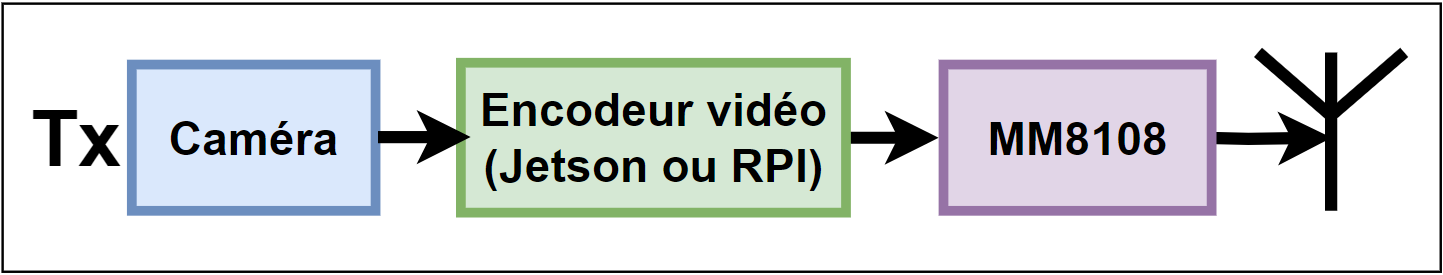
\includegraphics[width=0.7\linewidth]{imgs/Tx.png}
    \caption{Schéma Tx}
    \label{fig:Tx}
\end{figure}
    \item \textbf{Réception (RX) :} Module Wi-Fi Morse Micro MM8108 $\rightarrow$ Unité de routage (ex: OpenWrt, linux etc) $\rightarrow$ Unité de décodage et d'affichage (PC/Station au sol).
    \begin{figure}[H]
        \centering
        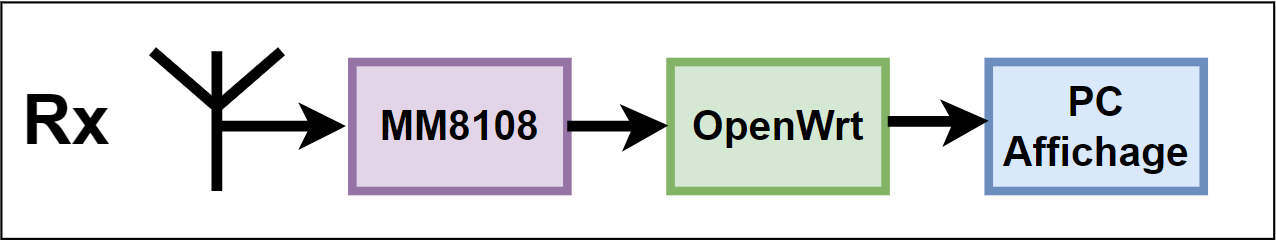
\includegraphics[width=0.7\linewidth]{imgs/Rx.png}
        \caption{Schéma Rx}
        \label{fig:Rx}
    \end{figure}
\end{itemize}